\section{Experimental Setup}
\label{expSetup}

%%%%%%%%%%%%%%%%%%%%%%%%%%%%%%%%%%%%%%%%%%%%%%%%%%%%%%%%%%%%%%%%%%%%%%%%%%%%%%%%%%%%%%%%%%%%%%%%%%%%%%%%%%%%%%%
%Initiator: Ran Itay
%Last modified by: MM Devi, May 26 2017
%Comment: The detector section has been modified. MMdevi's changes are made in blue
%%%%%%%%%%%%%%%%%%%%%%%%%%%%%%%%%%%%%%%%%%%%%%%%%%%%%%%%%%%%%%%%%%%%%%%%%%%%%%%%%%%%%%%%%%%%%%%%%%%%%%%%%%%%%%%
The experimental setup that is described in this section, is designed to measure, the spatial and 
temporal properties of LXe scintillation. However it is designed in a modular way, so it can serve different 
requirements from different future experiments. 

There are four main building blocks constructing the full setup, a schematics of them with the interfaces connecting them is shown in Fig.~\ref{fig:fullschematics}. The gas handling system, which, in normal working mode, drives the xenon from the detector trough a purifier and back into the detector. The cryogenic system, which liquefies the xenon and delivers it to the detector system. The detector system, mainly an HPFS sphere with a small bubble of LXe inside it surrounded with PMTs. Finally the data acquisition (DAQ) system that supplies high voltage (HV) and reads the data from all sensors (e.g., PMTs, pressure gauge etc.). Each building block can be replaced without effecting the others. 

\begin{figure}[t!]
\centerline{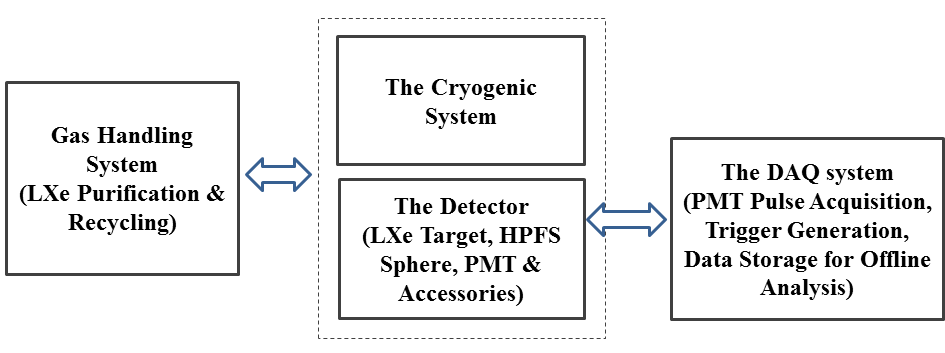
\includegraphics[width=0.8\linewidth]{WholeSys.png}}
\caption{A schematic of DIREXENO showing all the four building blocks of the system.}
\label{fig:fullschematics}
\end{figure}

The full assembly (Fig.~\ref{fig:fulldet}) is held on three separate racks, one for the DAQ, while the two others hold the cryogenic, detector and gas handling system. The racks are joined using a 100mm bar with shock absorbers on both sides. Some of the guidelines for the design of DIREXENO are based on~\cite{Giboni}  

\begin{figure}[t!]
\centerline{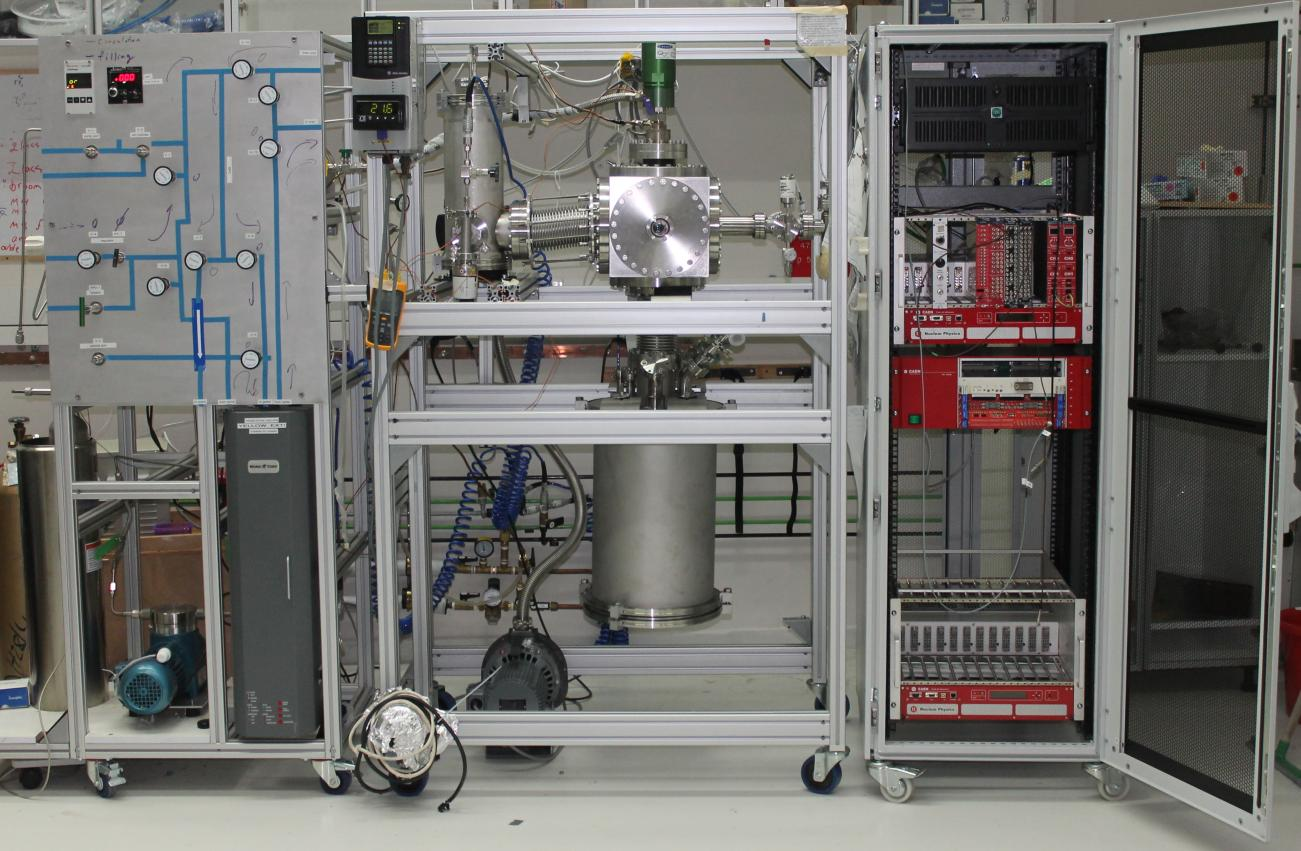
\includegraphics[width=0.8\linewidth]{FullDet.jpg}}
\caption{DIREXENO. On the left the purification system, in the middle the cryogenic and detector chamber, and on th right the Data acquisition system.}
\label{fig:fulldet}
\end{figure}

\subsection{Gas handling system}
\label{subsec:gas}

A typical LXe detector must keep a high level of purity. Careful selection and meticulously cleaning of all parts before mounting, is needed, however is not sufficient. The desired level of most detectors of impurity concentration is at the level of 1 ppb $O_2$ equivalent~\cite{Aprile:2009dv}. This is crucial to allow ionization electrons drift for several cm. To reach that level in a 
reasonable amount of time (several days instead of months), continuous purification is needed. The gas handling system, provides this process, 
alongside with all gas handling operations such as filling and recuperation.

During purification mode, xenon is taken from the chamber (in liquid phase)
passes through a heat exchanger\footnote{GEA GBS100M-24 plate heat exchanger} where it is heated and vapored. The xenon is forced 
by a KNF diaphragm pump into a hot getter\footnote{MONO-TORR
PS4-MT15-R-2} which cleans the xenon from most impurities. The xenon
also passes through an MKS Mass Flow Controller\footnote{MKS mass flow controller} (MFC), this allows monitoring and controlling the amount of xenon in the system. 

After the xenon is purified, it is delivered back to the cryogenic system through the heat exchanger, there the remained xenon gas is 
liquefied before it continuous back to the chamber. A schematic of this system is shown in fig.~\ref{fig:gasSchematic}.


\begin{figure}[t!]
\centerline{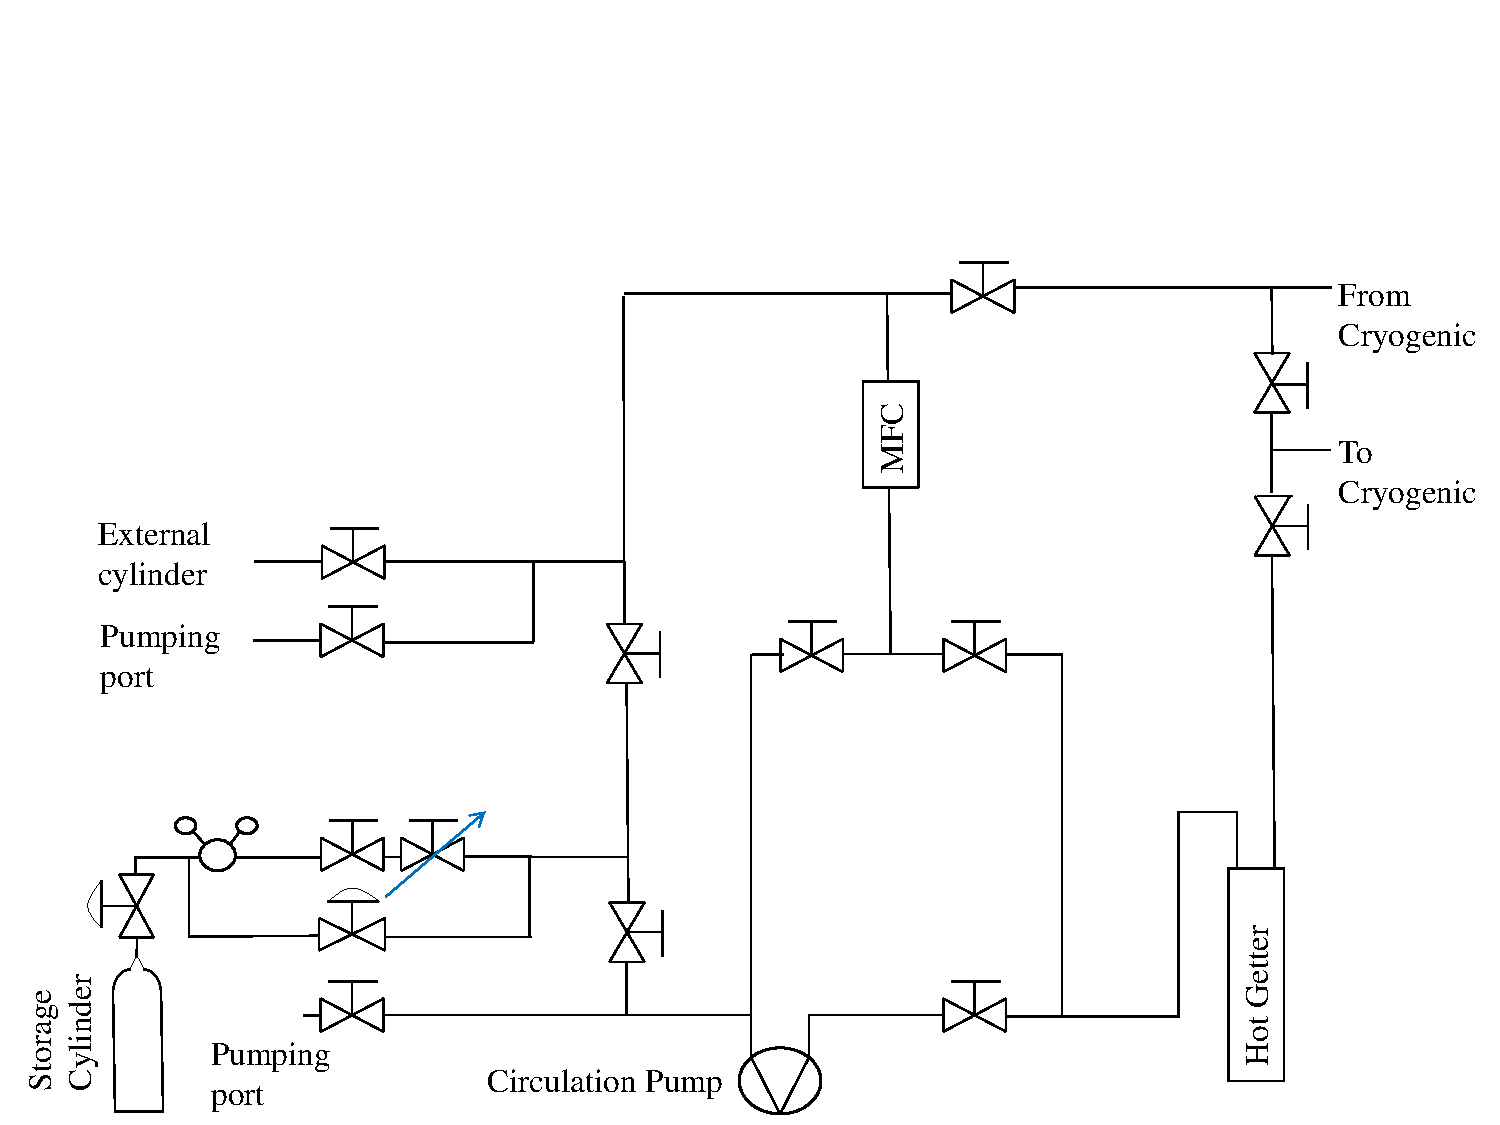
\includegraphics[width=1.\linewidth]{GasSchematics.pdf}}
\caption{Schematics of the purification system. High pressure valves are indicated as valves with arcs. Needle valves are indicated as 
a valve with an arrow.}
\label{fig:gasSchematic}
\end{figure}

\subsection{Cryogenic system}
\label{subsec:cryo}

Remote cooling is generally used in DM experiments due to background radiating from the cooler to the detector. Although in our system this is not of great importance there are still several advantages to remote cooling such as: lowering acoustic noise from the cryo-cooler and flexibility to design changes. The cryogenic system is connected on one side to the gas system and on the other to the detector chamber, any change in the system (e.g, cooler type or model) requires the change of that specific part without changing the detector nor the gas system.

The system is made out of two chambers, the outer vessel (OV) which holds the insulation vacuum, and the inner vessel (IV) that holds the xenon. In addition to the vacuum which prevents heat leaks from diffusion and convection, the entire IV is covered by multi layer aluminized Myler to prevent heating via radiation. An image of the detector and the CAD design are shown in Fig~\ref{fig:cryo}. 
\begin{figure}
	   \centering
	       \begin{subfigure}[c]{0.25\textheight}
		           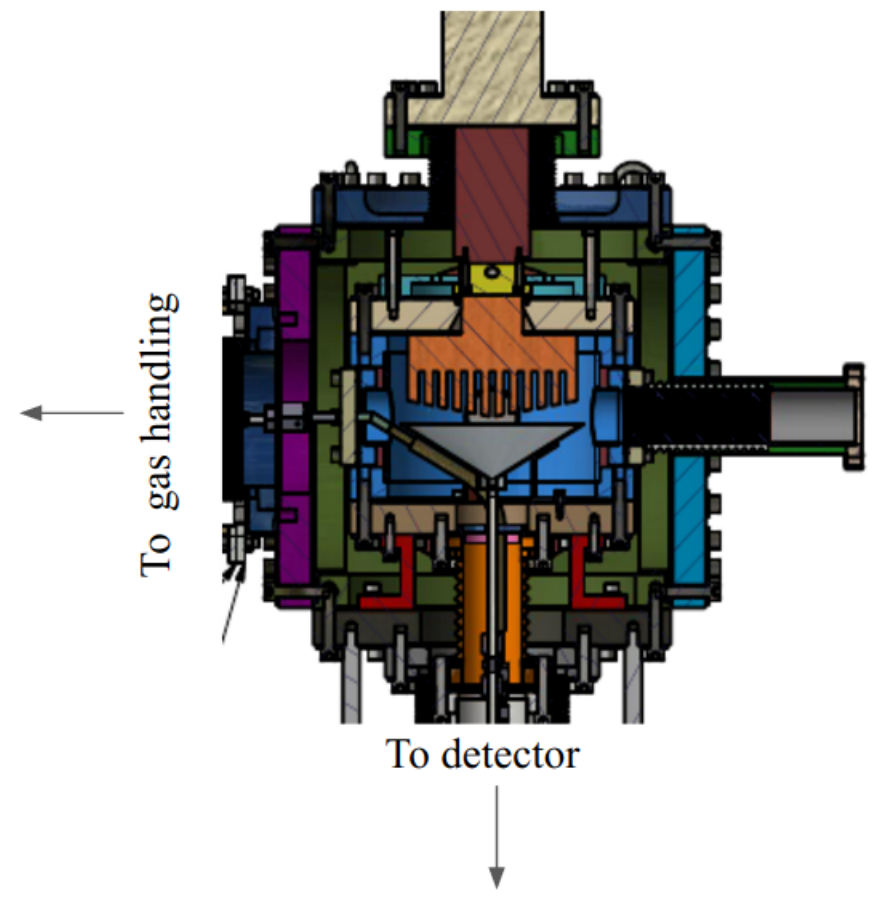
\includegraphics[width=\textwidth]{cryoMirror.png}
			       \end{subfigure}
			           \begin{subfigure}[c]{0.25\textheight}
					       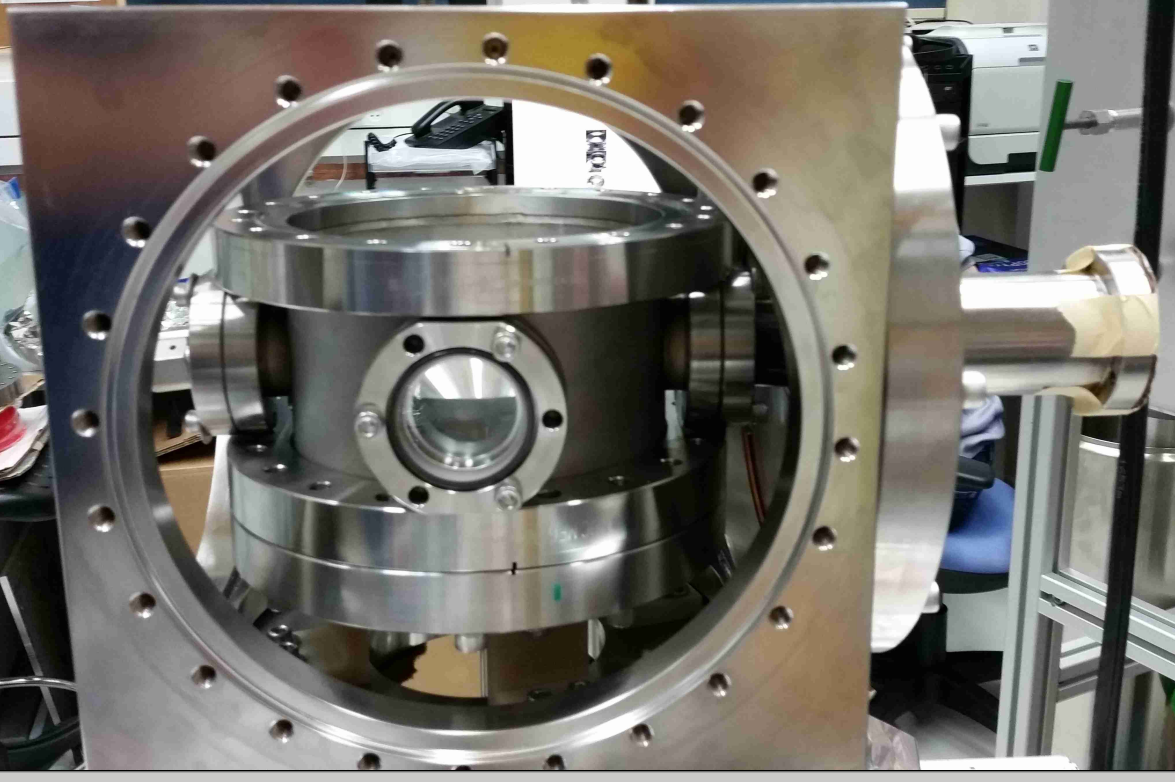
\includegraphics[width=\textwidth]{cryoOpenCrop.png}
					           \end{subfigure}
						           \caption{ CAD view of the cryogenic system(Left) and a pictue of the cryogenic system (Right) . \label{fig:cryo}}
						   \end{figure}

The OV is made of a 10" CF cube, with ports on all six faces (e.g., FT, pumping ports, view ports). This vacuum is shared with the detector one via a 6" CF flexible bellows.

The IV is made of 1.5" height cylinder with 6" CF flanges on the top and bottom parts of it, and it holds inside xenon. A 120~\,mm diameter cold finger is welded to the top flange of the IV, the inner part of the cold finger is made of long fins, therefore the surface area of it is bigger resulting in a better heat transport. The design of the cold finger is similar to the design of~\cite{xe100_instr2012}. The upper part of the cold finger is in thermal contact with the cryo-cooler~\footnote{QDrive 20BB 9p6 A 3 AYNBNCO} via a cooper adapter. The copper adapter holds two $100\Omega$ pt resistor which are connected to a PID reader\footnote{cryo-con model 18i Cryogenic Temp Monitor} for temperature measurements. A Cartridge-heater is also inserted to the copper adapter for emergency heating In case xenon freezes on the cold finger. 

The cryo-cooler provides up to 70 W of cooling power, and is connected via a $4\frac{1}{2}$" flange to the OV top flange, and reaching the IV top flange. 
Common cryo-coolers used for xenon experiments, work in maximal cooling mode permanently. The QDrive, instead, has temperature control allowing 
it vary the cooling power, which enables to set the temperature with fluctuations smaller then $0.1~\mathrm{C^{\circ}}$ on the cooler itself.

On the inner side of the bottom flange of the IV a thin 0.6~mm SS funnel is installed collecting all LXe drops from the cold finger, and delivering 
them to the  detector part. This flange is connected to the detector part, via a $3\frac{3}{8}$" flexible bellows. This bellows hosts two small pipes 
connected to the circulation system, and a third pipe coming from the funnel. All three pipes deliver LXe whereas the GXe is filling the bellows. The separation between the LXe coming from the gas handling system (clean) and the LXe coming from the cold finger (more dirty) allows the filling of clean LXe to different parts of the detector. 
%%%%%%%%%%%%%%%%%%%%%%%%%%%%%%%%%%%%%%%%%%%%%%%%%%%%%%%%%%%%%%%%%%%%%%%%%%%%%%%%%%%%%%%%%%%%%%%%%%%%%%%%%%%%%%%%%%%%%%%%%%%%%%%%%%%%%%%%%%%%%%%%%%%%%%%%%%%%%
\subsection{The Detector}
\label{subsec:det}
 

The detector refers to the chamber and its inner assembly that contains the liquid Xenon bubble, the photomultiplier detectors around it and their accessories. This chamber is placed below the cryogenic system. We describe the detector chamber and its interface to the cryogenic system in section \ref{subsubsec:detchamber}. In section \ref{subsubsec:sphere} we discuss the assembly 
that consists of the HPFS sphere to hold liquid Xenon and the Photomultiplier detectors distributed around the sphere.
\RanComment{The detector refers to the chamber and its inner assembly mainly an HPFS sphere that contains the liquid Xenon, the photomultiplier detectors around it and their accessories. This chamber is placed below the cryogenic system. We describe separately these two parts }
%%%%%%%%%%%%%%%%%%%%%%%%%%%%%%%%%%%%%%%%%%%%%%%%%%%%%%%%%%%%%%%%%%%%%%%%%%%%%%%%%%%%%%%%%%%%%%%%%%%%%%%%
\subsubsection{The Detector Chamber}
\label{subsubsec:detchamber}

The detector chamber is built such that apart from the interface to the cryogenic system, it can be changed and modified easily for future experiments.
The interface unit is built out of 2 flanges welded together via 7 tubes, which serve as service ports for electrical and other feedthroughs, 4 with a $2 \frac{3}{4}/$ CF flange, and 3 with a $1\frac{1}{3}$ CF flange. 
The upper flange, ISO-K NW320, is part of the OV and shares the insulation vacuum of the cryogenic system, the bottom one , CF-8", is 
part of an IV for future detectors, and would hold xenon inside. For our experiment we modified the CF flange to fit also a $4\frac{5}{8}$" CF 
flange which we use.

The OV is made of a ISO-K 320NW nipple closed with a blank from the bottom, the height of the nipple is determined such that the maximal height of the whole apparatus is 190~\,cm, allowing the mobility of the detector through standard doors.
 
The $4\frac{5}{8}$" CF flange is connected to a closed vessel internally divided into two parts. This vessel serves as a xenon reservoir. 
The two parts of the vessel are connected to a the HPFS sphere (see subcse~\ref{subsubsec:sphere}) from above (inner part) and from below (outer part). LXe is circulated such that new LXe drips into the outer part and pumped from the inner one. This way the liquid level is controlled, and the sphere itself is always filled with LXe. 



%%%%%%%%%%%%%%%%%%%%%%%%%%%%%%%%%%%%%%%%%%%%%%%%%%%%%%%%%%%%%%%%%%%%%%%%%%%%%%%%%%%%%%%%%%%%%%%%%%%%%%%%%%%%%%%%%%%%%%%
\subsubsection{The Sphere}
\label{subsubsec:sphere}

The central component of the detector assembly is \sout{the}\RanComment{a} hollow sphere which holds the LXe \sout{target} bubble. A spherical shell made of high purity fused silica with high transmittance is designed to hold the LXe target. \sout{The xenon will be circulated} Two invar tubes are connected to \sout{it}\RanComment{the HPFS sphere} from the top and bottom with 
SS mini-CF flanges at the end,\RanComment{. This allows xenon circulation through the sphere.} \sout{to circulate the xenon} (see Fig.~\ref{fig:sphere}). 

The bottom flange of the sphere is held using a brass holder to prevent force or torque applied on the sphere while mounting the detector. The 
brass holder is connected to a plate held from the top 8" flange, and is also used to align this plate at first installation. A set of 20 PMTs\footnote{r8520-406 Hamamatsu 1" PMT} are placed around the sphere to detect light emitted from the LXe.


The LXe target bubble should not be too large in order to avoid double scatters. The HPFS shell should be large enough to reduce internal reflections, but not too large \RanComment{to prevent attenuation o the scintillation light } \RanComment{which would attenuate the scintillation light}. The material of the shell should have a refractive index as similar to LXe as possible in order to have minimal diffraction from the original direction of the photons when they travel from the LXe target to the sphere. We chose corning HPFS 8655 as the shell material. The refractive index of HPFS 8655 is 1.575 at 185 nm (LXe R.I. 1.61). In Fig.~\ref{fig:hpfsRIcalibration}, are the refractive \RanComment{We need to check if indexes or indices as JINST is an American journal } indices at various wavelegths as given by the HPFS factsheet and also a naive extrapolation to lower wavelengths which are relevant to us. %and the transmittance 99.8\%/cm at 175 nm.

\begin{figure}
   \centering
   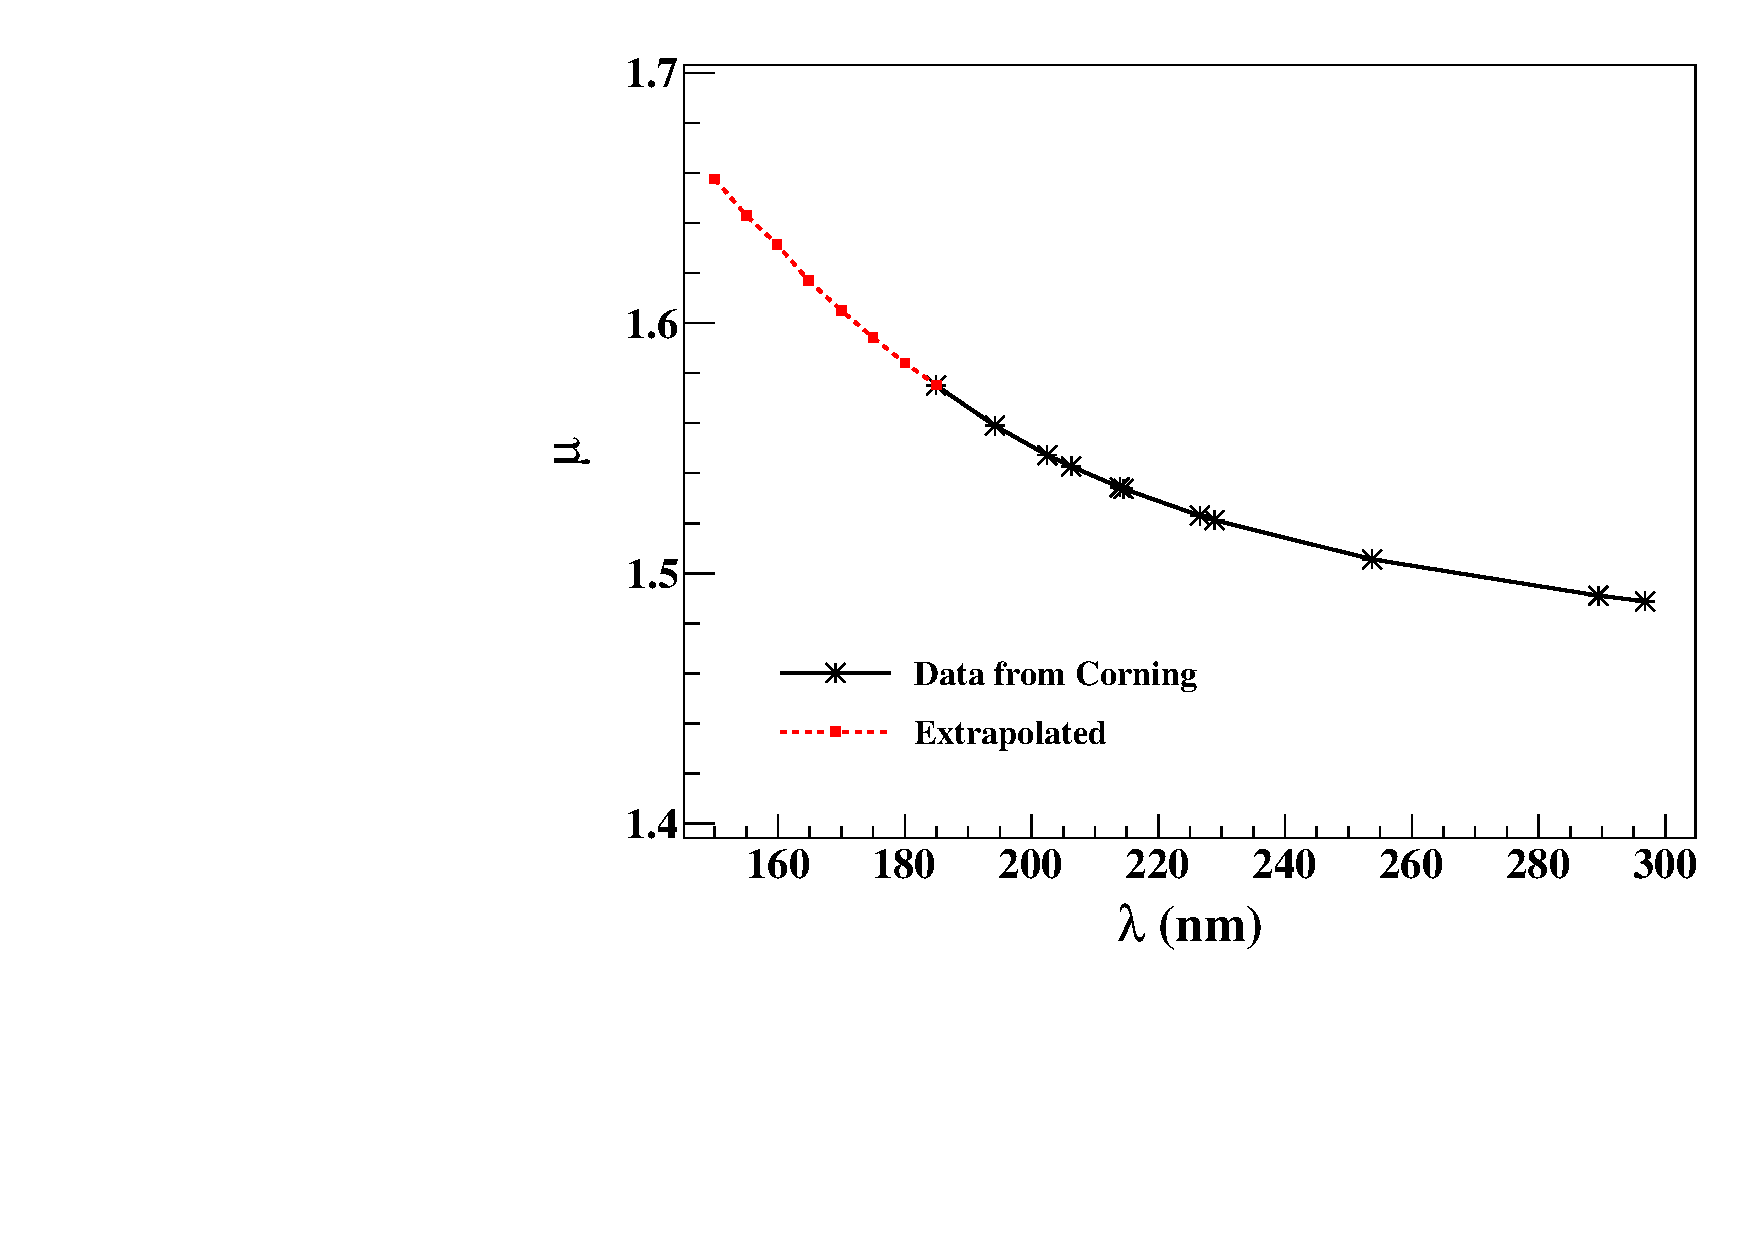
\includegraphics[width=0.48\textwidth]{RI-calibration.pdf}
    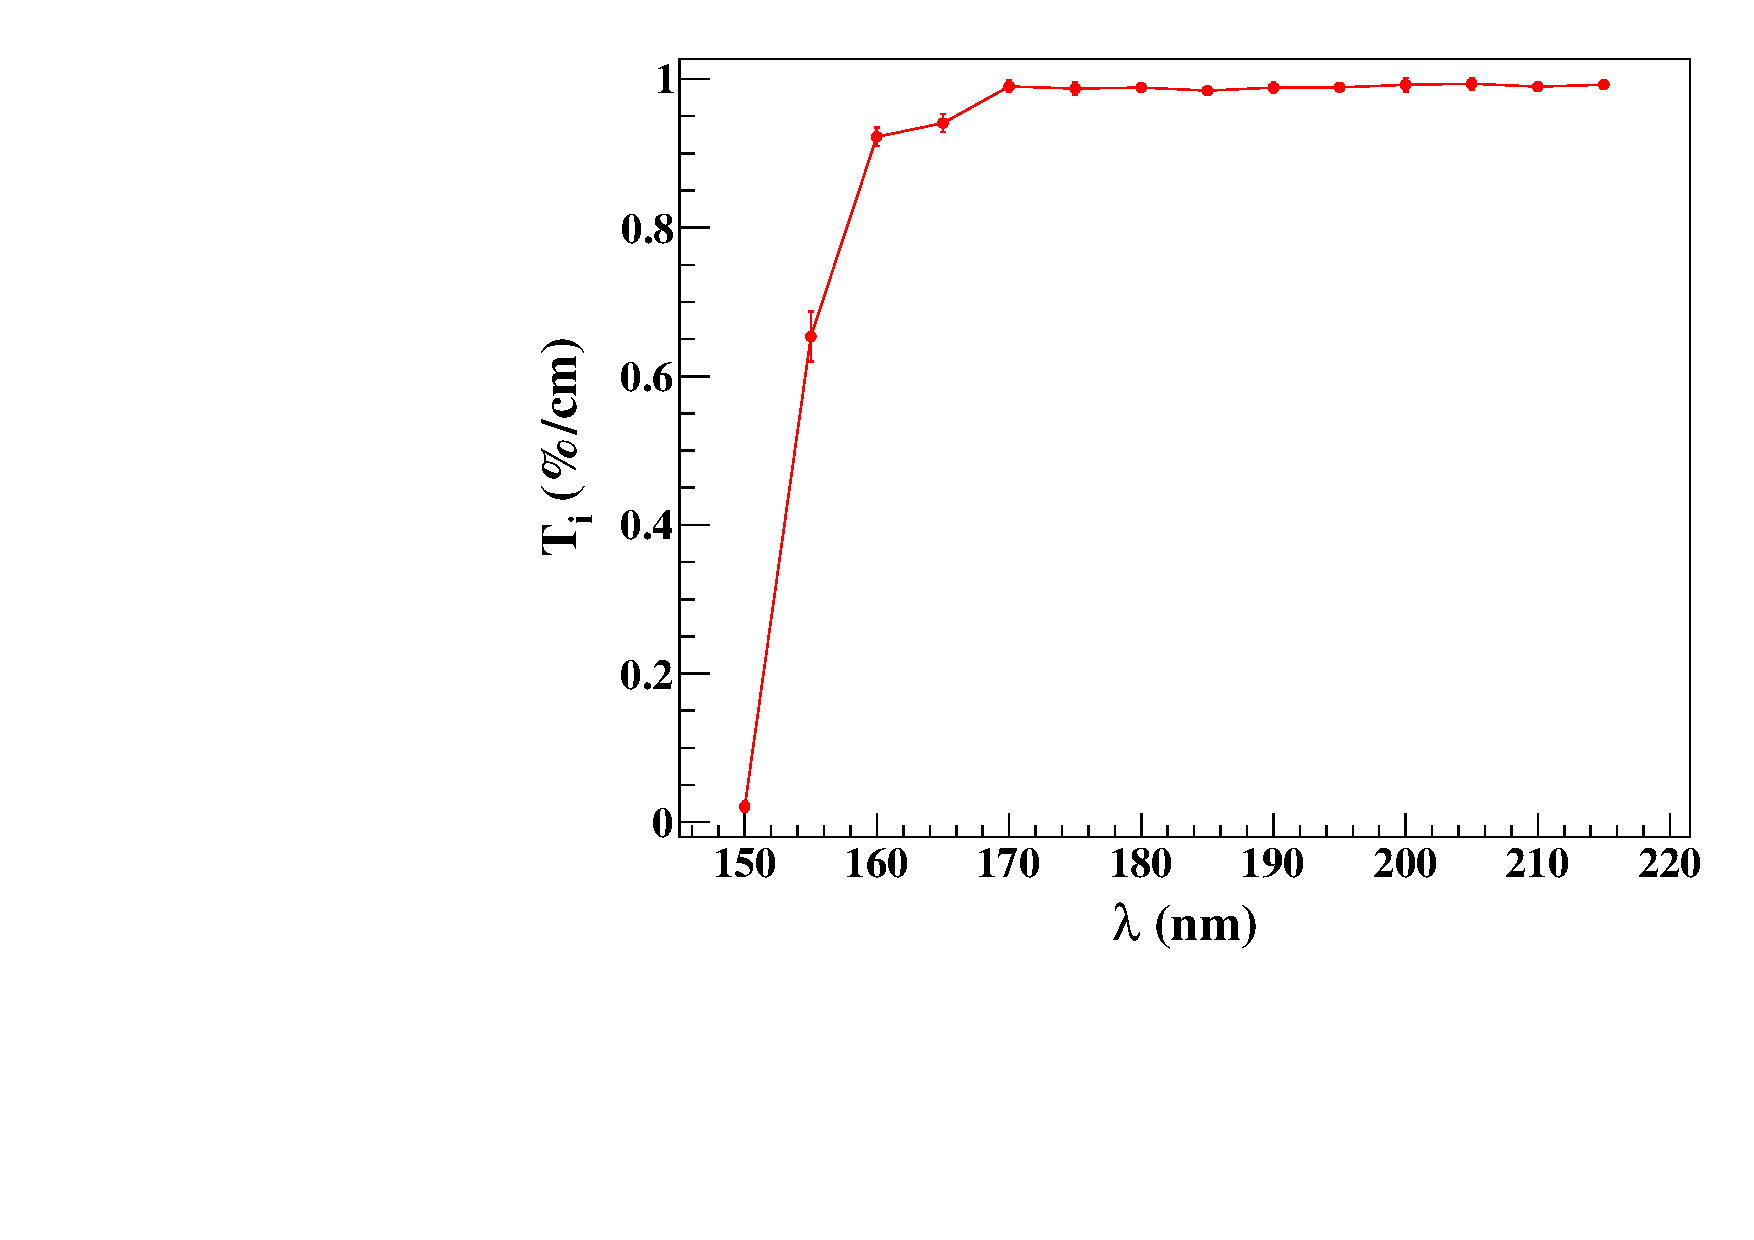
\includegraphics[width=0.48\textwidth]{IntTransmittance.pdf}
   \caption{The important characteristics of HPFS-8655. (Left) The refractive index as provided by corning and 
   extrapolated to relevant wavelength range. (Right) The internal transmittance ($T_{i}$).} 
   \label{fig:hpfsRIcalibration}
\end{figure}

The transmittance of the material is extremely crucial \sout{for us} to optimize the dimension of the shell. Therefore, \sout{we obtained} a 6 mm 
thick sample of HPFS 8655 \RanComment{test sample was obtained for transmittance test using a VUV monochromator} \sout{and performed a transmittance testing a VUV monochromator setup.} 
A deuterium light source was used to generate a spectrum in the range (110 - 950)~\,nm, peaked approximately at 160~\,nm. The window of the light source faced a vacuum space pumped to below $10^{-4}$ Torr. The monochromator allows to select the desired wavelengths using a manually rotatable holographic diffraction grating. A PMT placed in the vacuum measured the intensity of light emitted from the monochromator, with and without the fused silica sample. The ratio of measured intensities was used to calculate the transmittance of the material. In fig.~\ref{fig:transmittance} is the measured transmittances/ 6 mm at (150 - 215)~\,nm. At 175~\,nm the sample shows approximately 90\%/6mm measured transmittance which corresponds to an intrinsic transmittance of about 98\%.  \RanComment{Im not sure we need to specify the tests we did to measure the transmittance. I think we can just state that we did it using a VUV monochromator or something like that}


The dimension of the fused silica shell is optimized by studying the path of the scintillation photons using a GEANT4 based simulation~\cite{Agostinelli:2002hh}. The sources that will be used for exciting the xenon, and creating the supperradiance (signal) as well as the standard emission (background), will be $^{137} \mathrm{Cs}$ (662 keV) and $^{57} \mathrm{Co}$(122keV \& 136 keV) for ER and $^{241}$AmBe , D-D neutron generator, or neutron produced in an accelerator for NR . The mean free path for this energy is a couple of mm ($^{57} \mathrm{Co}$) and (0.5 - 3) cm ($^{137} Cs$).  \sout{We discuss the simulation in detail in section~\ref{sec:sim}}. 
The outer radius of the shell is 3 cm, while the inner radius of the hollow space that holds the LXe is 1 cm. \sout{The flow of the LXe will be maintained by two invar tubes}\RanComment{this is already explained above}. \RanComment{The technical design and a picture of the industrially manufactured shell assembly is shown in fig~\ref{fig:sphere}} In Fig.~\ref{fig:sphere} \sout{we show} 
the technical design and a picture of the industrially manufactured shell assembly. 



\begin{figure}
\centering
\begin{subfigure}[c]{0.4\textheight}
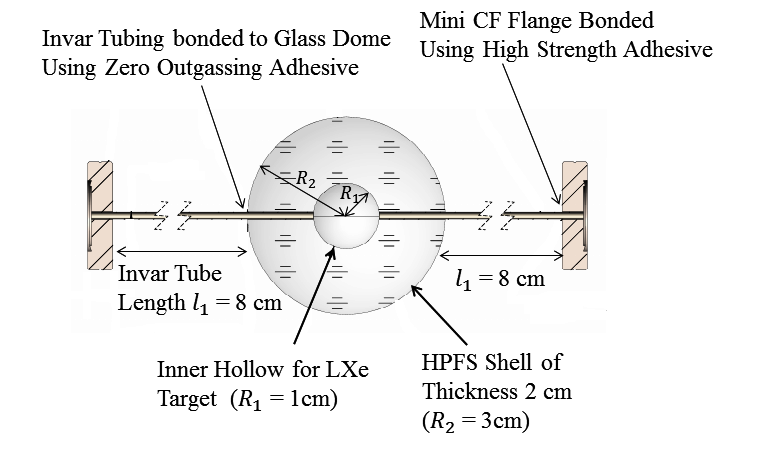
\includegraphics[width=\textwidth]{spheredesign1.png}
\end{subfigure}
\begin{subfigure}[c]{0.25\textheight}
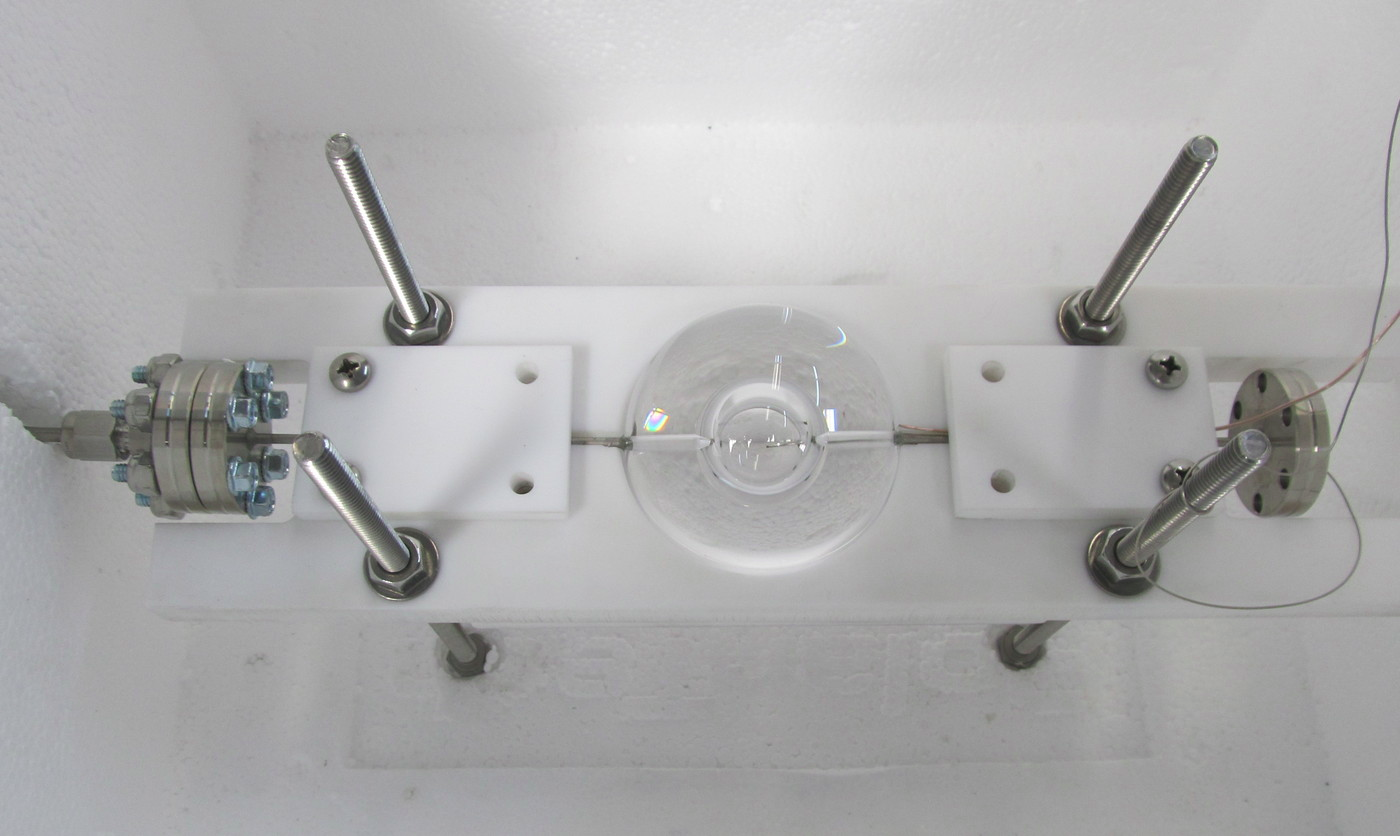
\includegraphics[width=\textwidth]{spherephoto.png}
\end{subfigure}
\caption{The technical design of the HPFS shell with invar tubing and flanges (left). The industrially manufactured
HPFS shell (right).} 
\label{fig:sphere}
\end{figure}


\sout{The p}Photons coming out of the system \sout{will be }\RanComment{are} detected by twenty 1'' square Hamamatsu R8520-406 PMT with an active area of 20.5 mm $\times$ 20.5 mm each. \sout{We pick the PMTs} \RanComment{The PMT are picked }  with a minimum quantum efficiency of 30\% at 178 nm. For an applied voltage of 900 V the gain of these PMTs are ~ 2 $\times$ 10$^6$. We use a positive voltage divider, also manufactured by Hamamatsu, to provide high voltage to the PMTs. These 20 PMTs are held with a special aluminum holder, coated with anti-reflection substance. The holder is made of two hemispheres hosting the PMTs in 
3 rows all of them pointing to the center of the fused-silica sphere. the PMTs are held only via their voltage--divider bases. 
The bases are held using M2 PEEK screws. 
In Fig.~\ref{fig:pmtholder}, one of the holder--hemispheres with the PMTs are shown.

\begin{figure}
   \centering
   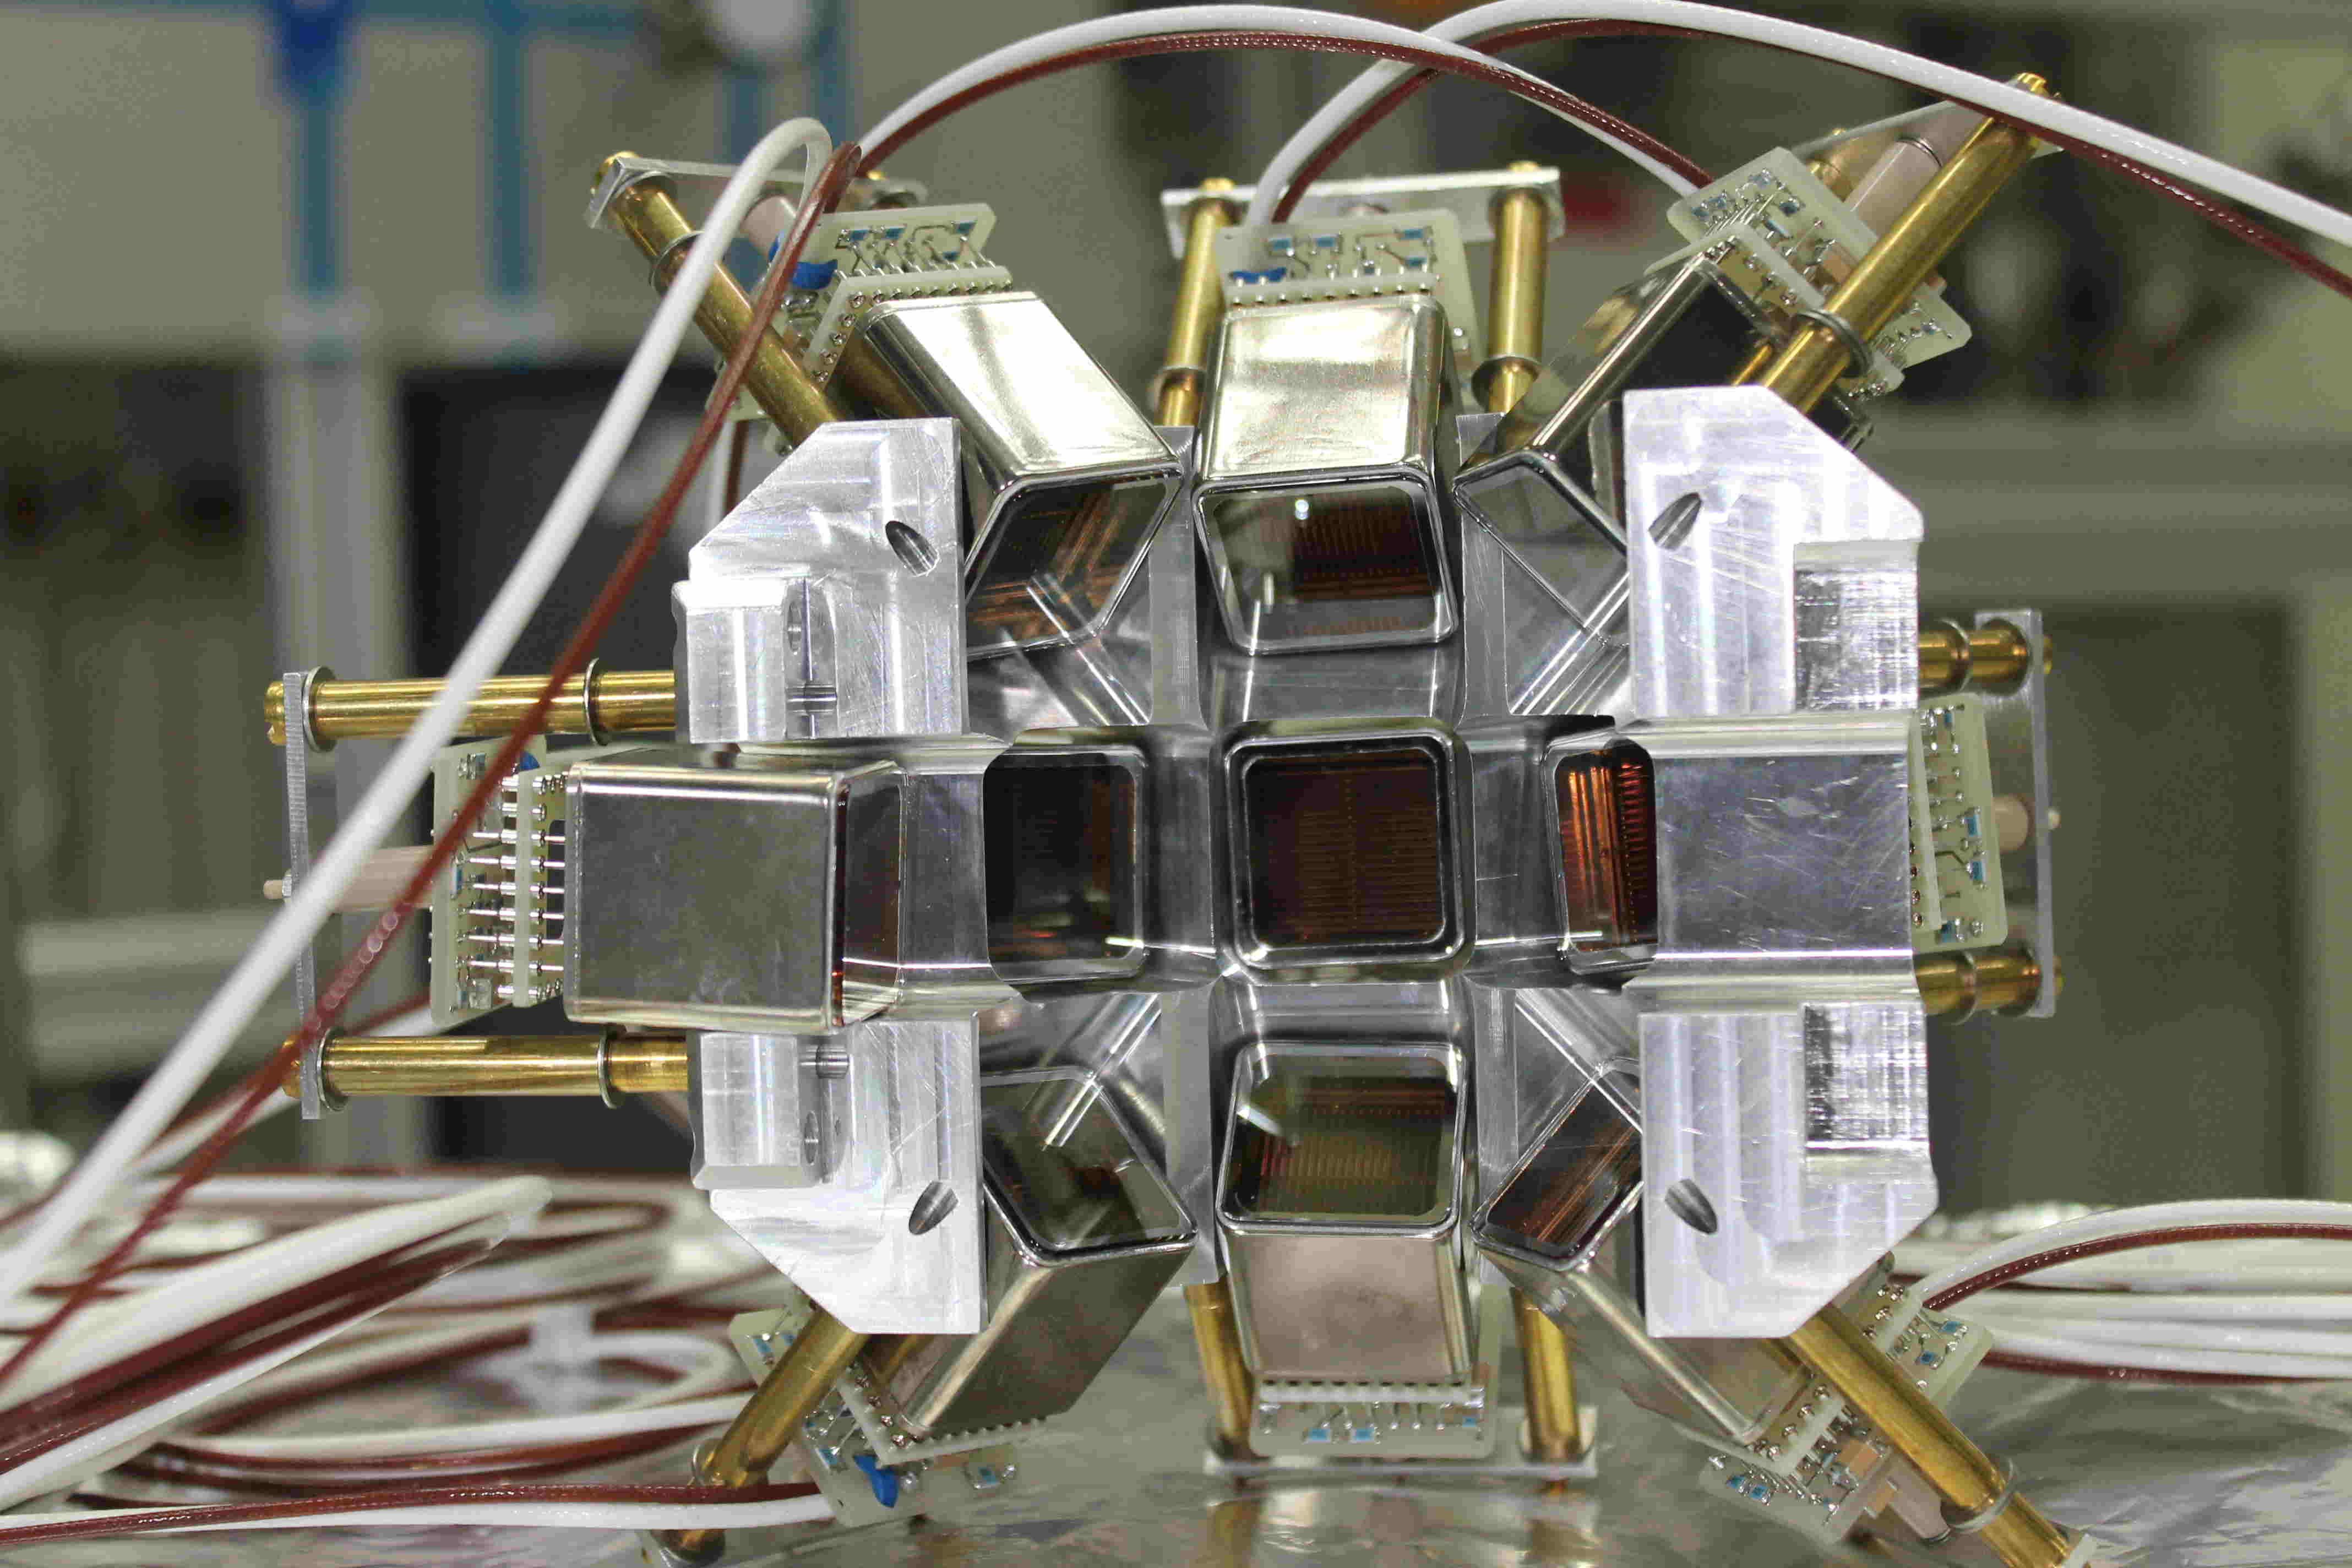
\includegraphics[width=0.5\textwidth]{PMTholder.JPG}
   \caption{A PMT holder--hemisphere. We use two such components to hold 20 PMTS around the target.} 
   \label{fig:pmtholder}
\end{figure}


%\clearpage %temporary MMD
In Fig.~\ref{fig:detector} we present a CAD schematic as well as a real view of the detector part.

%%%%%%%%%%%%%%%%%%%%%%%%%%%%%%%%%%%%%%%%%%%%%%%%%%%%%%%%%%%%%%%%%%%%%%%%%%
\begin{figure}
	\centering
    \begin{subfigure}[c]{0.45\textwidth}
		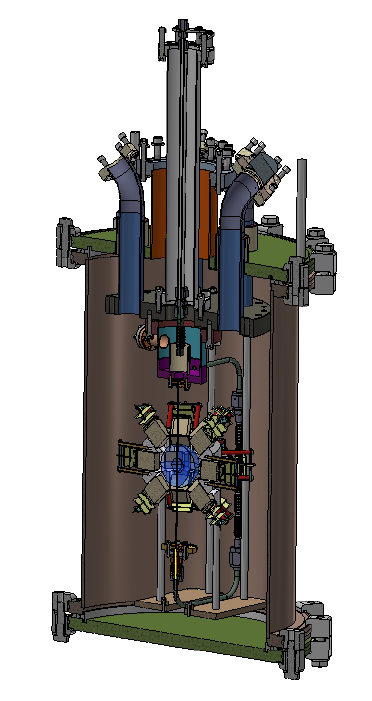
\includegraphics[width=0.75\textwidth , height=0.3\textheight]{detCAD.png}% Here is how to import 
	\end{subfigure}	
	\begin{subfigure}[c]{0.45\textwidth}
		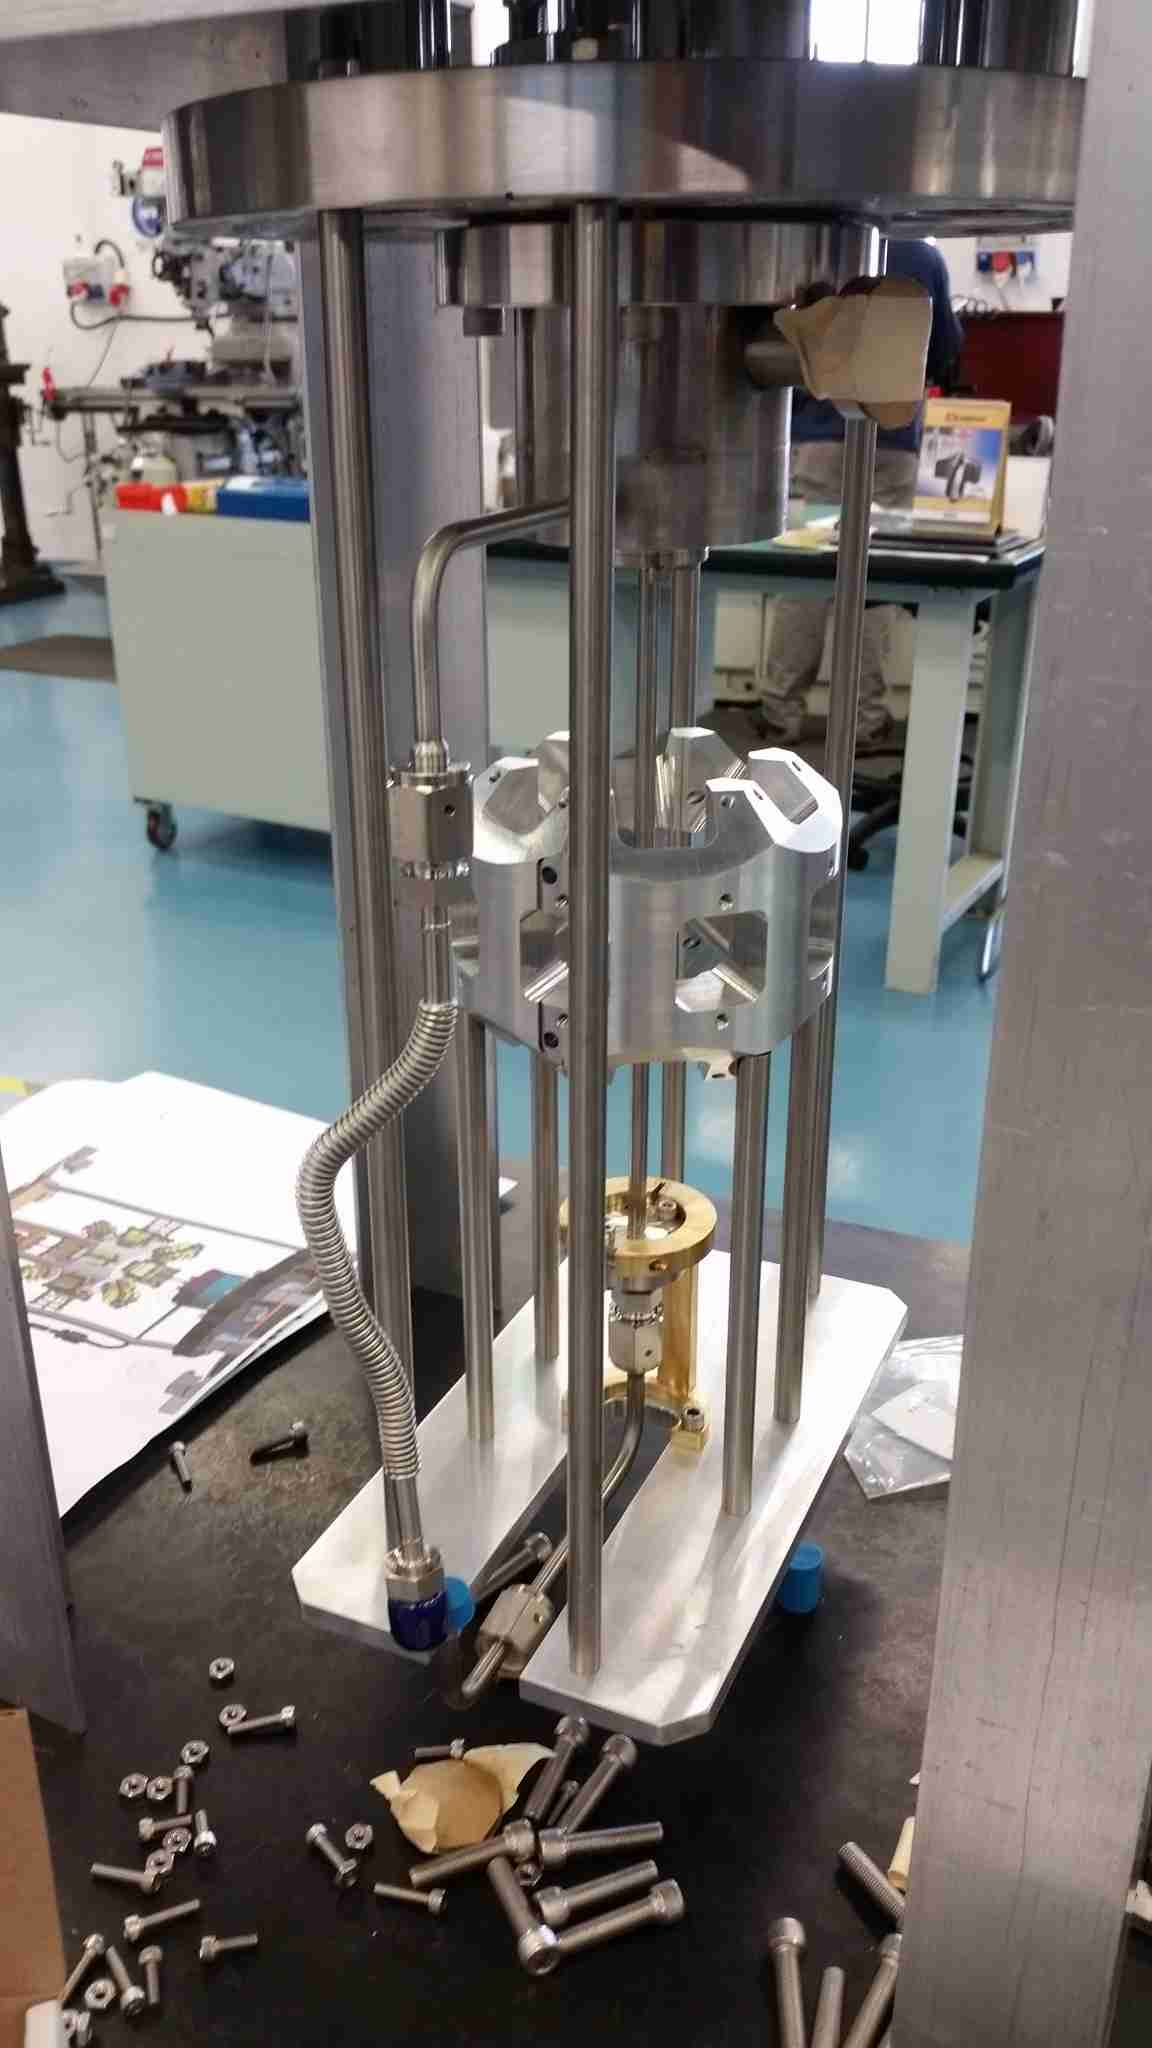
\includegraphics[width=\textwidth , height=0.3\textheight]{detReal_small.jpg}% Here is how to import 
	\end{subfigure}	
		\caption{\label{fig:detector} (Left) CAD design of the detector part. (Right) First mounting of the 
		detector part, still not connected to the rest of the system.}
	
\end{figure}
%%%%%%%%%%%%%%%%%%%%%%%%%%%%%%%%%%%%%%%%%%%%%%%%%%%%%%%%%%%%%%%%%%%%%%%%%%%%
